\documentclass[a4paper]{jarticle}
\usepackage[dvipdfmx, hiresbb]{graphicx}
\usepackage[top=30truemm, bottom=30truemm, left=30truemm, right=30truemm]{geometry}
\usepackage{float}
\usepackage{ascmac}
\usepackage{amsmath}
\usepackage{amssymb}
\usepackage{bm}
\usepackage{amsfonts}
\usepackage{here}
\begin{document}
\title{ファクター・リスク寄与度に基づく\\ポートフォリオの構築について\\}
\author{東京理科大学工学部経営工学科 \quad 黒木 裕鷹}
\maketitle
%%%%%%%%%%%%%%%%%%%%%%%%%%%%%%%%%%%%%%%%%%%%%%%%%%%%%%%%%%%%%%%%%アブスト
\begin{abstract}

運用期間が数カ月程度の短期間で投資パフォーマンスを得るために,近年盛んに研究されているマルチ・ファクターモデルを用いたポートフォリオを構築した.
Fama-Frenchの3ファクターモデルに代表されるマルチ・ファクターモデルでは,ファクターの選択方法や学習データに対して過学習してしまう問題が指摘される.
また,ファクター選択の適切さやファクター間の相関がもたらす交絡などによる影響は,マルチ・ファクターモデルの重要な課題である.

株価は時系列データであり,その性質上新たに観測されるデータは常に将来のデータであるため,予測が困難である.
たとえば,時系列に関するモデリングではモデルの複雑化にともなうオーバーフィッティングの影響を非常に受けやすい.
本レポートではこの問題を解決するため,モデル推定では近年パターン認識の分野でしきりに利用されているlasso回帰を用い,最適なパラメータの選択には交差検証法を用いた.
推定したマルチ・ファクターモデルからファクター・リターンに対する銘柄の影響度を算出し,特異なパフォーマンスを示す銘柄を投資対象としてポートフォリオに組み込む手法を提案した.

バックテストでは,提案したマルチ・ファクターモデルと手法を用いて構築したポートフォリオが長期的に安定してベンチマーク(日経225やTOPIX)をアウトパフォームする結果となった. 
これはファクターのリスク・プレミアムを上手く抽出できた結果であると考えられ,同様の戦略によるポートフォリオをBloomberg Global Investment Contestにおいて提出した.
\end{abstract}



\newpage
\pagenumbering{roman}
\newpage
\tableofcontents

\newpage

\listoftables

\listoffigures
\newpage



\pagenumbering{arabic} 



%%%%%%%%%%%%%%%%%%%%%%%%%%%%%%%%%%%%%%%%%%%%%%%%%%%%%%%%%%%%%%%%%%%初めに
\section{はじめに}
金融資産の運用では,どのように各資産の将来価格を予測するのかが重要な課題となる.
株価の将来価格の予測は,
1) ファンダメンタルズ分析に基づく手法,
2) テクニカル分析に基づく手法,
3)統計モデルによる手法,
を用いて行われるのが一般的である.
このようにアプローチの仕方は様々存在するが,企業や投資家にとって,将来の株価予測モデルの構築は金融資産運用を行う上で重要な課題である.
本レポートではBloomberg投資コンテストに向け無裁定価格理論(APT)とマルチ・ファクターモデルによる株価収益率モデルを構築し,ポートフォリオ運用に応用する.

\subsection{Bloomberg投資コンテスト}
本コンテストで行うシミュレーションは一般的に行われている金融取引とは異なる.最終的な目標は一定のルールのもとでより高い収益を獲得することであるため,投資の戦略もルールに基づいたものでなくてはならない.ルールを概観し,以下にまとめた.

\begin{enumerate}
\item ルール
\begin{enumerate}
\item ポートフォリオ登録時点で時価総額が1億円以内になるように登録
\item 10銘柄以上,30銘柄以下でのポートフォリオを構成
\item 2017年7月31日までであれば1度だけ銘柄の入れ替え(リバランス)が可能
\item ロングポジションのみ(空売り禁止)
\item 手数料は考慮しない
\end{enumerate}

\item パフォーマンス計測期間
\begin{enumerate}
\item  2017年7月3日 $\sim$ 2017年8月31日
\end{enumerate}

\item パフォーマンス測定方法
\begin{enumerate}
\item ポートフォリオ機能「トータルリターン(\%)」を頻度日次・円建てで計測
\item ポートフォリオ登録は登録日より2営業日前の終値をコスト価格として登録
\item ポートフォリオ登録後,6月中の価格変動による時価総額の増減を含め7月3日から8月31日の間でパフォーマンスを計測
\end{enumerate}
\end{enumerate}

以上のルールの中で,時間的な制約は1-c, 2-aである.これらにより1か月単位のバイアンドホールドを強いられ,さらにルール3-bにより終値での取引に限定され,鞘取りを行うことは困難である.
つまり,長期的な視点から価格変動のメカニズムを考察し,どの銘柄をポートフォリオに組み込むのか,という問題を考えなければならない.
次節では,価格変動の源泉について考察した.

\subsection{価格変動の源泉}


金融資産は一般的な商品と異なり,投資目的やリスクヘッジ目的で購入されることがほとんどである.
そのため資産価格は需要供給の関係だけでなく価格変動の予想にも影響される.
株式市場が効率的であるという効率的市場仮説のもとでは,あらゆる「情報」が株価形成に瞬時に反映されているはずであるため,それらの「情報」を用いた将来価格の予測は不可能ということになる.
%証券投資理論を見て加筆する???
一方,テクニカル分析に基づく株価予測モデルは,株価の将来価格は過去の株価の変動パターンから予測可能であるという仮定のもとに用いられる.
一般の投資家は株式市場で適切な価格形成が行われているか,自力で十分な情報を得ることが出来ないため,将来価格の予測に使用できる「情報」が存在する.
たとえば,アナリストによる予測やレポートがある.
しかしアナリストやテクニカル指標による株価予測の情報は,
1) 検証することが困難,
2) バイアンドホールドによる運用には向かない,
などの理由から,本レポートでは考察の対象としない.
本研究では,株価はAPTにより決定されると仮定した統計モデルによる予測を試みる.

\subsection{CAPMとAPT}
株式市場に上場している様々な企業は,それぞれが異なった価格変動の性質を持っている.
企業の経営方針や持っている技術,リリースしている商品,組織体系などが多種多様であるためだ.
しかし,複数の企業に共通している性質も考えられる.
例えば所属国や業種,企業の規模などだ.
このような共通の要因(ファクター)のうち,株価の変動に関係を持つものが存在する可能性は十分にある.
ファクターモデルとは,株価変動のある部分は共通要因の変動によって説明可能である,とするモデルである.

資産価格変動の共通要因を考えた理論として最も広く知られているものの一つは,ウィリアム・シャープらによる資本資産価格モデル(Capital Asset Pricing Model : CAPM)だろう.
市場ポートフォリオを唯一の共通要因とした資産価格の評価手法である.
CAPMは1960年代より不動の地位を築き,その計算の簡便さもあり現在でも広く用いられている.
しかし1970年代以降,CAPMに対する様々な批判や問題点が提起され,代わりとなる新たな理論が提唱されてきた.
株価変動の共通要因は複数存在すると仮定したマルチ・ファクターモデルである.


最も代表的なマルチ・ファクターモデルはFama-Frenchの3ファクターモデル\cite{Fama}だろう.
このモデルを構築したファーマとフレンチは米市場における実証分析を行い,企業規模(Size)や簿価比時価率(Value)が株価の収益構造に関与していると結論付けた.
企業規模の小さい銘柄や,時価総額が総資産額に比べて割安な銘柄は平均的に高い収益を見せることを示したのである.
この現象はそれぞれ小型株効果,バリュー株効果と呼ばれ,CAPMにおける代表的なアノマリー(説明できない事象)として認識されている.
ファーマとフレンチはその功績により2013年にノーベル経済学賞を受賞している.
実際に似たような性質(業種や企業規模など)を持つ銘柄は似たような価格変動を見せることが多く,ファーマとフレンチが対象とした米市場に限らず,金融資産の価格変動が市場ポートフォリオ以外のファクターにも影響されているという主張は自然なものだと考えられる.
実際,多くの先進国市場を対象にしたFama-Frenchの3ファクターモデルの有用性が報告されている.

また,ファクターモデルと密接に関わる理論としてステファン・ロスの無裁定価格理論(APT)\cite{Ross}がある.
APTはCAPMと異なり,全資産の収益率の同時分布が正規分布であることを必要しない.
APTが必要とする仮定は,「投資家はただ飯をいくらでも食べたがる」という,ほぼ自明の行動原理のみである\cite{analyst}.
そのためAPTはCAPMよりも柔軟な理論として知られている.

\subsection{投資戦略の決定}

マルチ・ファクターモデルとAPTにより,CAPMよりも確からしい資産の価格変動の構造を考え,それを応用した運用手法を提案することを目標にする.
また,本コンテストのパフォーマンス測定は2カ月間のみの短いものであり,偶発的な金融危機については考えないこととする.
とはいえ収益に見合わないリスクを持つポートフォリオを構成することには利点がないため,特に理由がない限り構成銘柄数は最大の30銘柄を考える.

マルチ・ファクターモデルにより各銘柄の収益構造を推定した後の問題はポートフォリオに組み込む資産をどのように選択するかである.
投資には必ずリスクが伴い,投資家はそのリスクを代償にリターンを求める.
そこでここでは,それぞれのファクターの持つリスクに晒される「価値」を考えることとした.
この「価値」は通常リスク・プレミアムと呼ばれる.高いリスク・プレミアムを持つファクターに対してリスクを取り,低いリスク・プレミアムを持つファクターに対して分散化することを考えていく.

\subsection{レポート構成}
本レポートの2章ではポートフォリオ構築に使用した諸理論や既存のモデルを体系だてて述べる.
3章では実際に行ったデータ解析の手順を述べ,バックテストの結果と共に提案する手法を示す.
4章では提出したポートフォリオの途中経過を示し,行ったリバランスについても触れる.
5章では提案手法に対する課題の提示と,まとめを行う.









%%%%%%%%%%%%%%%%%%%%%%%%%%%%%%%%%%%%%%%%%%%%%%%%%%%%%%%%2章

\section{ファクターモデルに基づくポートフォリオ選択}

ポートフォリオ構築の基盤とした理論や,参考にした既存のモデルについて述べる.なお,金融工学に基づく基本的な理論は文献\cite{analyst}\cite{finance}を参考にした.


\subsection{シングル・ファクターモデルとしてのCAPM}
市場を構成する資産数を$N$とする.CAPMの枠組みにおいて金融資産$i$の収益率$r_i$は,唯一の共通要因(シングル・ファクター)である市場ポートフォリオの収益率$R_M$に依存する変動と,資産特有の変動$\varepsilon_i$に分けられ以下の式(\ref{eq:CAPM})ように表される.また,資産特有の変動$\varepsilon_i$は資産間で相互に無相関であると仮定される.$r_f$は無リスク利子率を表す定数であり,信用の高い長期国債の年利が一般的に用いられる.
\begin{equation}
\begin{split}
&r_i - r_f = \alpha_i + \beta_i(R_M - r_f) + \varepsilon_i,\qquad(i=1,\cdots,N)\\
&\varepsilon_i \sim i.i.d.N(0,\sigma_i^2),\\
&Cov(R_M, \varepsilon_i) = 0,\\
&Cov(r_i, r_j) = 0, \qquad (i \neq j)
\label{eq:CAPM}
\end{split}
\end{equation}
ここで,$\beta_i$は金融資産$i$の市場ポートフォリオへの感度を表し,$\alpha_i$は市場ポートフォリオに対する期待超過収益率を表している.式(\ref{eq:CAPM})より$r_i$の分散を求めると
\begin{equation}
Var(r_i) = \beta_i^2Var(R_M) + Var(\varepsilon_i) \qquad (\text{∵}Cov(R_M, \varepsilon_i) = 0)
\label{eq:CAPM_var}
\end{equation}
となる.この右辺第1項はシステマティック・リスクと呼ばれ市場ポートフォリオの動きにより説明可能な部分である.
また右辺第2項は企業固有のアンシステマティック・リスクと呼ばれる.

これらのリスクのうち,アンシステマティック・リスクはポートフォリオ選択によって除去可能であるとしばしば言われる.
このことを見るために,式(\ref{eq:CAPM})により記述される資産を用いた空売り禁止のポートフォリオを考える.
資産$i(i=1,\cdots,N)$の保有比率が$w_i$であるようなポートフォリオ$P$の収益率$R_P$は以下で与えられることになる.ただし,$\sum_{i=1}^N w_i = 1, w_i\geq0$である.
\begin{equation}
\begin{split}
R_P &= \alpha_P + \beta_PR_M + \varepsilon_P\\
&= \sum_{i=1}^N w_i\alpha_i
+\left(\sum_{i=1}^N w_i\beta_i\right)R_M
+\sum_{i=1}^N w_i\varepsilon_i
\end{split}
\end{equation}
また,このポートフォリオの分散は以下で与えられる.
\begin{equation}
\begin{split}
Var(R_P) &= \beta_P^2 Var(R_M) + Var(\varepsilon_P)\\
& = \left(\sum_{i=1}^N w_i\beta_i\right)^2Var(R_M) + \sum_{i=1}^N w_i^2 Var(\varepsilon_i)
\label{eq:var_port}
\end{split}
\end{equation}
この$\beta_P$がポートフォリオの市場ポートフォリオに対する感度になり,$\alpha_P$がポートフォリオの市場ポートフォリオに対する期待超過収益率となる.ここで,式(\ref{eq:var_port})の右辺第2項がポートフォリオのアンシステマティック・リスクである.$0\leq w_i \leq 1$であることより,以下の式が成立する.
\begin{equation}
\sum_{i=1}^N w_i^2Var(\varepsilon_i) \leq \sum_{i=1}^N w_iVar(\varepsilon_i)
\end{equation}
つまり,アンシステマティック・リスク$Var(\varepsilon_i)$が銘柄ごとに大差ない場合,十分分散化されたポートフォリオのアンシステマティック・リスクは,各資産のアンシステマティック・リスクに比べ非常に小さくなる.



\subsection{CAPMに対する批判}
1.3節で述べたように,CAPMに対しては様々な批判が為され,実証分析が行われてきた.以下にその代表的なものを挙げる.
\begin{itemize}
\item Basu(1977)\cite{Basu}\\
ニューヨーク証券取引所において,株価収益率(PER)の低い銘柄が高い銘柄に比べて良いパフォーマンスを見せることを実証した.
\item Banz(1981)\cite{Banz}\\
企業規模の小さい銘柄が大きい銘柄に比べて良いパフォーマンスを見せることを実証した.
\item Jagadeesh and Titman(1993)\cite{Jagadeesh}\\
モメンタムの強い銘柄が市場をけん引し続ける傾向があることを実証した.
\end{itemize}

ファクターモデルによるアンシステマティック・リスクはポートフォリオ選択によって除去可能であると言われてきたが,これが不可能であることをいずれの研究も示している.企業特有の撹乱項が企業ごとに独立ではなく,共分散が影響しているということである.マーケット以外の共通要因も存在しうることを示唆している.CAPMの枠組みでは,市場ポートフォリオによって説明できる部分(市場ベータ)と出来ない部分(アルファ)に分けられ,超過収益であるアルファはポートフォリオ・マネージャーの手腕によるものたと解釈されてきた.しかし次節で述べるマルチ・ファクターモデルの発見により,マネージャーの手腕によると言える部分は徐々に減り,代わりにファクターのリスク・プレミアムによる部分が増えることとなった.

以下の図\ref{fig:beta}にそのイメージを示した.
左から1番目の棒グラフはポートフォリオ収益率全体を表している.2番目の棒グラフはCAPMの$R_P=\alpha_P + \beta_PR_M$,3番目は$R_P = \alpha_P + \beta_{market}F_{market} + \beta_{size}F_{size}$,4番目は$R_P = \alpha_P + \beta_{market}F_{market} + \beta_{size}F_{size} + \beta_{value}F_{value}$とモデル化したときの収益構造のイメージ図である.

\begin{figure}[H]
	\begin{center}
		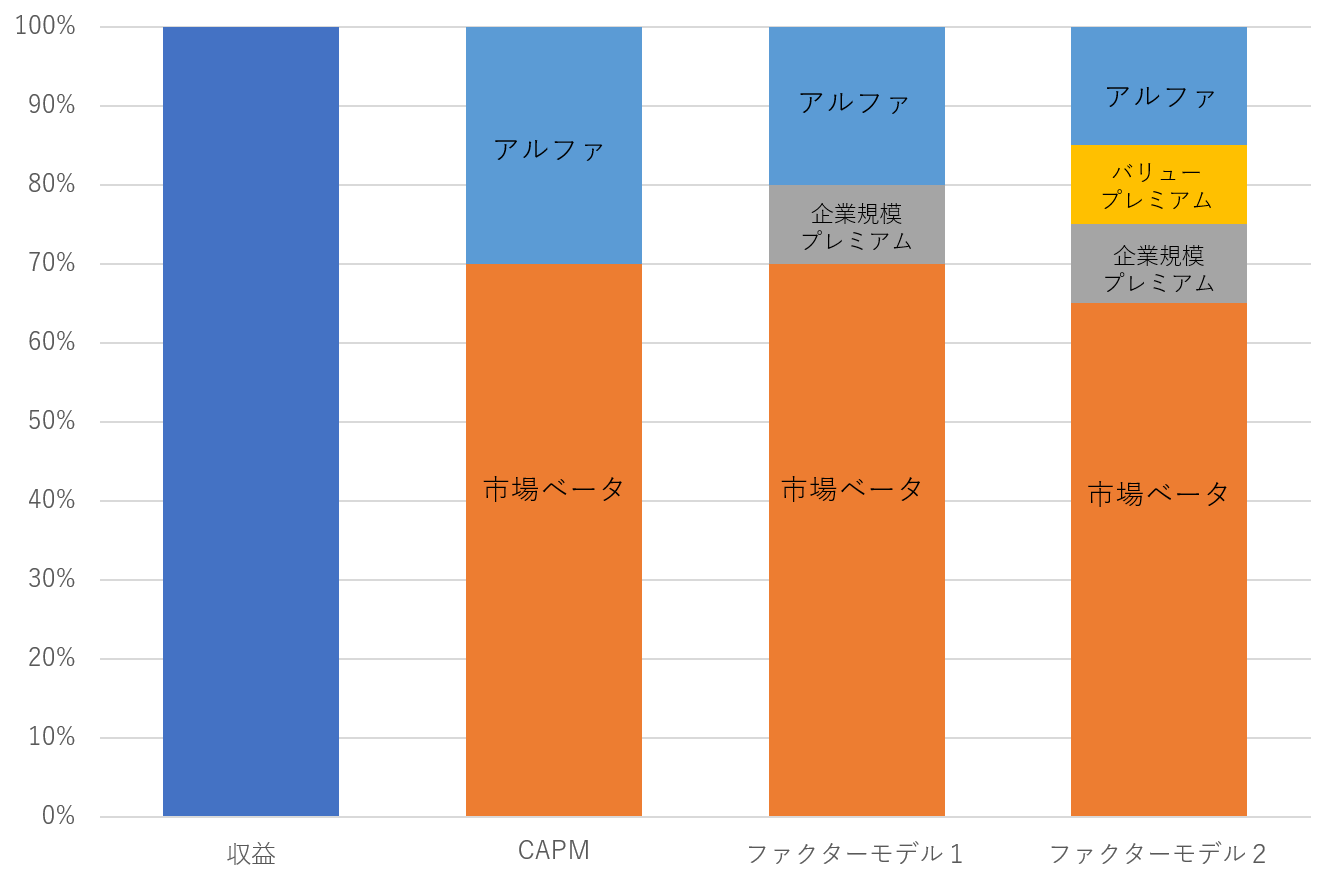
\includegraphics[width=14cm]{./fig/beta}
		\caption{モデル別にみた収益構造}
		\label{fig:beta}
	\end{center}
\end{figure}




\subsection{マルチ・ファクターモデル}
ここでは,各資産の収益率が$m$個の共通要因に依存するマルチ・ファクターモデルを考える.金融資産$i$の収益率$r_i$は企業特有の部分$\varepsilon_i$と共通要因であるファクター$F_k(k=1,\cdots,m)$によって決定される.また,$\varepsilon_i$は資産間で相互に無相関であると仮定すると,$r_i$は以下のように表される.
\begin{equation}
r_i = \alpha_i + \beta_{i,1}F_1 + \beta_{i,2}F_2 + \cdots + \beta_{i,k}F_k + \cdots + \beta_{i,m}F_m + \varepsilon_i
\label{eq:multifactor}
\end{equation}
ここで,2.1節と同様,資産$i(i=1,\cdots,N)$の保有比率が$w_i$であるようなポートフォリオ$P$の収益率$R_P$を考えると以下のようになる.
\begin{equation}
\begin{split}
R_P &= \alpha_P + \beta_{P,1} F_1 + \beta_{P,2} F_2 + \cdots + \beta_{P,m} F_m + \varepsilon_P\\
&=\sum_{i=1}^N \alpha_i + F_1 \sum_{i=1}^N w_i \beta_{i,1} + \cdots + F_m \sum_{i=1}^N w_i \beta_{i,m} + \sum_{i=1}^N w_i\varepsilon_i\\
&= \sum_{i=1}^N \alpha_i + \sum_{k=1}^m \sum_{i=1}^N w_i \beta_{i,k} F_k + \sum_{i=1}^N w_i\varepsilon_i
\label{eq:multi}
\end{split}
\end{equation}

%次に,式(\ref{eq:multi})の分散を考える.
%ポートフォリオの分散は求めたほうが良いの?

\subsection{APT}

\subsubsection{仮定}
APTでは,金融資産の価格構造がファクターモデルで表されることを仮定する.
ここでは一般形として,任意の資産$i$の収益率は式(\ref{eq:multifactor})のように表され,$\varepsilon_i$は資産間で相互で無相関であるとする.
またAPTでは追加として,各ファクターの期待値が0でなければならない.
これは,あらかじめ使用するファクターを正規化することにより解決する.
以上APTの仮定についてまとめたものを以下に示した.

\begin{itembox}[l]{APTの仮定}
各資産$i$の収益率は以下のように表される.
\begin{eqnarray}
& r_i = \alpha_i + \beta_{i,1}F_1 + \cdots + \beta_{i,k}F_k + \cdots + \beta_{i,m}F_m + \varepsilon_i\label{eq:APT_return} \\
& E(\varepsilon_i) = 0 \qquad (i=1,2,\cdots,N)\\
& E(F_k) = 0 \qquad (k=1,2,\cdots,m)\\
& Cov(\varepsilon_i, \varepsilon_j) = 0 \qquad (i \neq j) \label{eq:APT_cov}
\end{eqnarray}
\end{itembox}
ここで,式(\ref{eq:APT_return})について期待値を取ると
\begin{equation}
E(r_i) = \alpha_i
\end{equation}
となる.つまり,式(\ref{eq:APT_return})における定数項は資産$i$の期待収益率に相当する.
ファクターモデルを仮定しているので,複数の資産で構成されるポートフォリオの収益率は式(\ref{eq:multi})と同様に記述される.
ここで,式(\ref{eq:APT_cov})により,ポートフォリオが十分な数の資産で構成されるとき,$\varepsilon_P$は無視しても構わない.
つまり,十分に分散化されたポートフォリオの収益は,ファクターに対する感度のベクトル$(\beta_{P,1},\cdots,\beta_{P,m})$によってのみ特徴づけられる.




\subsubsection{APTの主定理}
APTの発想は,市場に裁定機会がないというものであった.
無数の市場参加者が存在することによって裁定取引は常に行われ,適正でない金融資産の価格は裁定取引のできない水準に収束することになる.
これはノー・フリーランチの原理と呼ばれる.
この原理を価格理論に応用することにより,APTの主定理が導かれる.十分に分散化されていれば,ファクターへの感度が全く同じになっているポートフォリオ同士のリターンは同じでなければならない,ということである.

\begin{itembox}[l]{APTの主定理}
証券の収益率がマルチ・ファクターモデルで表されるとする.
このとき,任意の資産$i$の各ファクターへの感度を$(\beta_{i,1},\beta_{i,2},\cdots,\beta_{i,m})$とすると,資産$i$のリスク・プレミアムは
\begin{equation}
\lambda_1\beta_{i,1} + \lambda_2\beta_{i,2} + \cdots + \lambda_m\beta_{i,m}
\label{eq:APT}
\end{equation}
で近似的に表される.ただし,$( \lambda_1, \lambda_2, \cdots ,\lambda_m )$は各ファクターのリスク・プレミアムである.
\end{itembox}
%証明いる???

\subsubsection{ファクターのリスク・プレミアムの推定}
APTの主定理で用いるファクターのリスク・プレミアムの推定について触れる.
資産を組み合わせて,特定のファクターへの感度のみが1で,その他のファクターへの感度が0になるポートフォリオ(ファクター・ポートフォリオ)を考える .例えば,第1ファクターのみへの感度が1になるようなポートフォリオを$P_1$とすると,その収益率は
\begin{equation}
R_{P_1} = \alpha_{P_1} + 1\times F_1 + 0\times F_2 + \cdots + 0\times F_m + \varepsilon_{P_1} 
\end{equation}
と表せる.このとき,$\alpha_{P_1}$が第1ファクターの期待収益率であり,リスク・プレミアムとなる.

一般に,$m$個のファクターを想定すると,単一ファクター・ポートフォリオの収益率ベクトルは
\begin{equation}
\left(
	\begin{array}{cccc}
	R_{P1}\\
	R_{P2}\\
	\vdots \\
	R_{Pm}
	\end{array}
\right)
=
\left(
	\begin{array}{cccc}
	\alpha_{P1}\\
	\alpha_{P2}\\
	\vdots \\
	\alpha_{Pm}
	\end{array}
\right)
+
\left(
	\begin{array}{cccc}
	1 & 0 & \ldots & 0\\
	0 & 1 & \ldots & 0\\
	\vdots & \vdots & \ddots & \vdots \\
	0 & 0 & \ldots & 1
	\end{array}
\right)
\left(
	\begin{array}{cccc}
	F_1 \\
	F_2 \\
	\vdots \\
	F_m
	\end{array}
\right)
+
\left(
	\begin{array}{cccc}
	\varepsilon_{P1}\\
	\varepsilon_{P2}\\
	\vdots \\
	\varepsilon_{Pm}\\
	\end{array}
\right)
\end{equation}
と表される.行列ベクトル表記すれば次式のようになる.
\begin{equation}
\mbox{\boldmath $R$}_P = \mbox{\boldmath $\alpha$}_P + \mbox{\boldmath $I$}_m\mbox{\boldmath $F$} + \mbox{\boldmath $\varepsilon$}_P
\end{equation}
となる.この単位行列$\mbox{\boldmath $I$}_m$は,ファクターモデルの係数行列$\hat{\bm{B}}$($\hat{・}$は推定値を表す)と未知の荷重行列$\mbox{\boldmath $W$}$の積で表現できると仮定する.


第$k(k=1,2,\cdots,m)$ファクターに対する感度のみが1であるポートフォリオを第kファクター・ポートフォリオ$P_k$とし,$P_k$における資産$i$のウェートを$w_{i,k}$とする.さらに,資産$i$の第$k$ファクターへの感度を$\hat{\beta_{i,k}}$とすると,以下の式(\ref{eq:fp})を\mbox{\boldmath $w$}について解くことによりファクター・ポートフォリオを構築できる.



\begin{equation}
\mbox{\boldmath $W$}^\text{T} \hat{\bm{B}} = \mbox{\boldmath $I_m$}
\label{eq:fp}
\end{equation}
式(\ref{eq:fp})左辺の$\beta_{i,k}$による感度行列は式(\ref{eq:multi})により推定されるので,$w_{i,k}$によるウェート行列が求める対象である.感度行列の逆行列を左辺の右からかければ良いことになるが,感度行列の型は$n\times m$であり,正方行列ではない.
しかしこれは一般化逆行列$\hat{\bm{B}}^\dag$を用いることにより解決する.
ただし,$\hat{\bm{B}}^\dag = (\hat{\bm{B}}^\text{T}\hat{\bm{B}}^{-1})\hat{\bm{B}}^\text{T}$である.







\section{データ解析}
\subsection{使用したデータ}
2015年1月から2017年5月にかけて,東証一部上場企業の株価と各指数を日次終値を取得した.なお,データの取得にはBloomberg端末とMicrosoft ExcelのBloombergアドインを使用し,データ分析はR言語により行った.
\begin{itemize}
\item 投資対象市場の選択について\\
\quad 東証一部上場企業の株式の価格データを使用した.\\
\quad 数々の先行研究により,CAPMだけでなくマルチ・ファクターモデルにおいても市場ポートフォリオが第1の共通要因になることに疑いの余地はない.
そこで分析を行いやすくするため対象ユニバースは一つに絞ることを考え,馴染みの深い日本の東京証券取引所の株式を選択した.
また東証二部や東証マザーズに関して,流動性の不十分性よりマルチ・ファクターモデルが十分な説明力を発揮しない可能性があるため,除外することとした.
\item ファクターについて\\
マルチ・ファクターモデルを構成する際,以下のファクターを使用した.
\begin{itemize}
\item マーケット・ファクター\\
東証一部上場銘柄を対象としているため,マーケットファクターとしては東証一部上場銘柄の時価総額を反映しているTOPIXを使用した.マーケットファクターの収益率には対数収益率を用いた.
\item サイズ・ファクター\\
Russell/Nomuraの提供する日本株インデックスで代用した.具体的には,配当を含めないSmall Cap Indexから配当を含めないLarge Cap Indexを引くことにより算出した.さらにその変動をみるために差分を取ったものを使用した.
\item バリュー・ファクター\\
Russell/Nomuraの提供する日本株インデックスで代用した.具体的には,配当を含めないTotal Value Indexから配当を含めないTotal Growth Indexを引くことにより算出した.さらにその変動をみるために差分を取ったものを使用した.
\item 為替ファクター\\
日本円(JPY)の市場価格(対米ドル)を為替ファクターとして使用した.さらにその変動をみるために対数差分を取ったものを使用した.
\item 市場ボラティリティ・ファクター\\
S\&PがVIXと同様の手法で算出している日本市場における30日インプライド・ボラティリティを使用した.
\end{itemize}
上記のファクターはそれぞれ単位もスケールも異なるので,正規化(平均0分散1に標準化)した後に使用した.\\
\quad 
サイズ・ファクターとバリュー・ファクターについては先行研究が豊富であり,その存在はほぼ確実とされている.
%竹原などによる日本におけるFama-Frenchを参考文献に挙げる
次に為替ファクターであるが,これは日本市場が主にアメリカ市場から影響を受けることに起因する.
%VARモデルによる分析入れる?
マーケット・ファクターが為替ファクターを包含しているのではないか,という疑問は持たれるだろうが,業種や海外進出の有無などによりその感度は銘柄ごとに異なるだろう.
そのため円ドル相場をファクターとして取り入れることとした.
最後にボラティリティ・ファクターについてであるが,これは低ボラティリティ・ファクターとは異なるものである.
というのも投資家たちは市場ボラティリティの大きさに従い,リスクを調整するためにリバランスを行うが,その際に取引が集中する銘柄を検出しようと狙ったものである.
このとき,資産価格はボラティリティの変動というよりもその大きさに影響されると考えられるため,差分を取らずに日経VIX系列を正規化した.\\
%モメンタム・ファクターは取り入れなかった.3カ月間で一つのモデル推定をしたため,アルファが柔軟に吸収してくれる.

\end{itemize}



\subsection{データのクリーニング・概観}
分析対象期間の2015年1月から2017年5月において,何らかの理由(未上場等)により継続的にデータが取得できない企業を除外した.分析対象の1948企業に対し,さらに対数差分をとることによって各営業日の日次対数収益率を算出した.

対象銘柄すべての価格推移をプロットすることは紙面の都合上割愛した.
%%%%%%%%%%%%%%%%%%%%%%%%%%%%%リスク・リターン平面書ければ書く.
ファクターに関しては,前節のように各指数を加工した後に使用する.
原系列である各指数について確認するため,Bloomberg端末にて該当期間のラインチャートを取得し,エクスポートしたものを以下の図\ref{fig:TOPIX}から図\ref{fig:Value}に示した.
図\ref{fig:TOPIX}はTOPIXの原系列である.ファクターには対数差分を正規化したものを使用した.
\begin{figure}[H]
	\begin{center}
		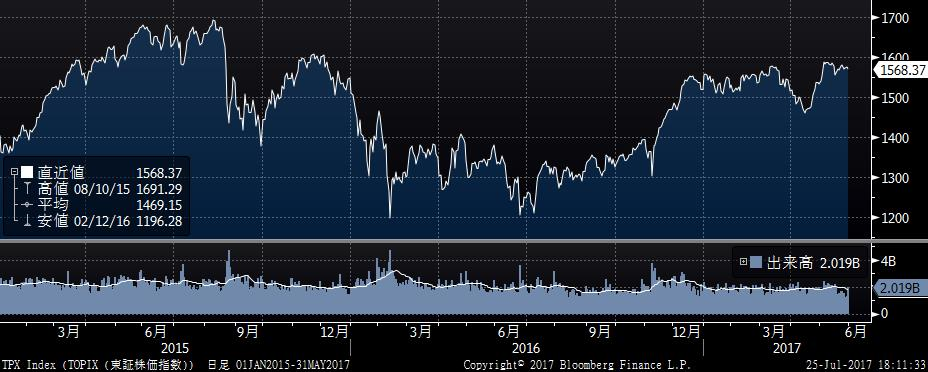
\includegraphics[width=15cm]{./fig/TOPIX.jpg}
		\caption{TOPIXの時系列プロット}
		\label{fig:TOPIX}
	\end{center}
\end{figure}
図\ref{fig:VIX_JPY}の上段が日本円レート(対米ドル),下段がS\&Pが提供する日経VIXの原系列である.日経VIXは正規化したものを,日本円レートは対数差分を正規化したものをファクターとして使用した.
\begin{figure}[H]
	\begin{center}
		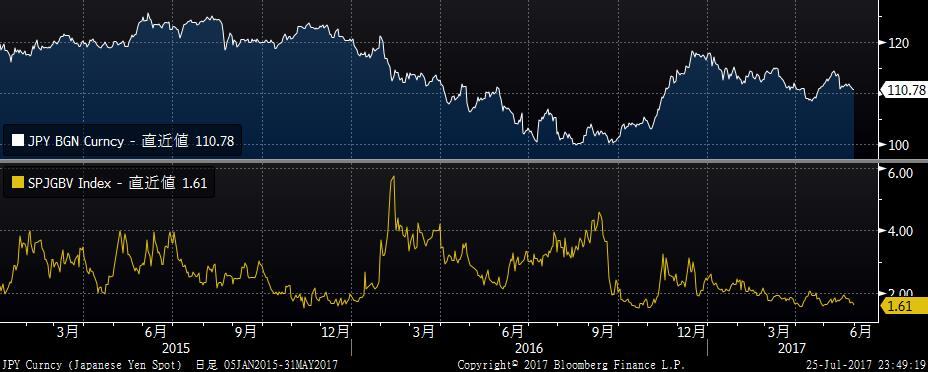
\includegraphics[width=15cm]{./fig/VIX_JPY.jpg}
		\caption{日本円レートと日経VIXの時系列プロット}
		\label{fig:VIX_JPY}
	\end{center}
\end{figure}
図\ref{fig:Size}の上段がRussell Nomuraの提供する日本小型株インデックスと日本大型株インデックス,下段が日本小型株インデックスから日本大型株インデックスを減算したものである.ファクターには下段の差分を正規化したものを使用した.
\begin{figure}[H]
	\begin{center}
		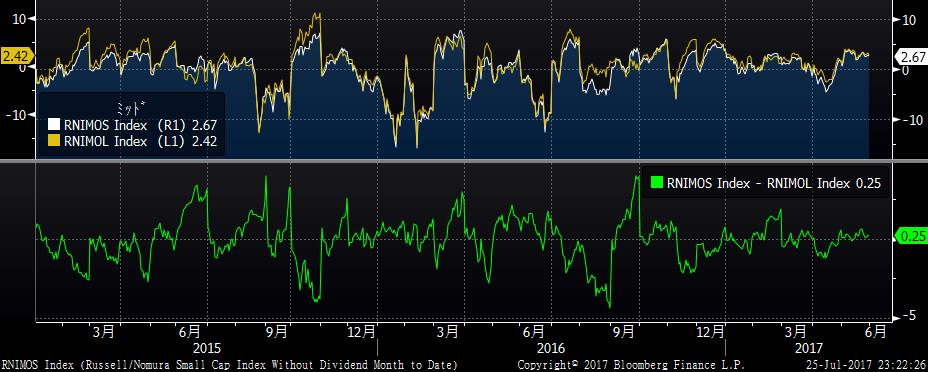
\includegraphics[width=15cm]{./fig/Size.jpg}
		\caption{Russell Nomura日本株インデックス(Size)}
		\label{fig:Size}
	\end{center}
\end{figure}
図\ref{fig:Value}の上段がRussell Nomuraの提供する日本バリュー株インデックスと日本グロース株インデックス,下段が日本バリュー株インデックスから日本グロース株インデックスを減算したものである.ファクターには下段の差分を正規化したものを使用した.
\begin{figure}[H]
	\begin{center}
		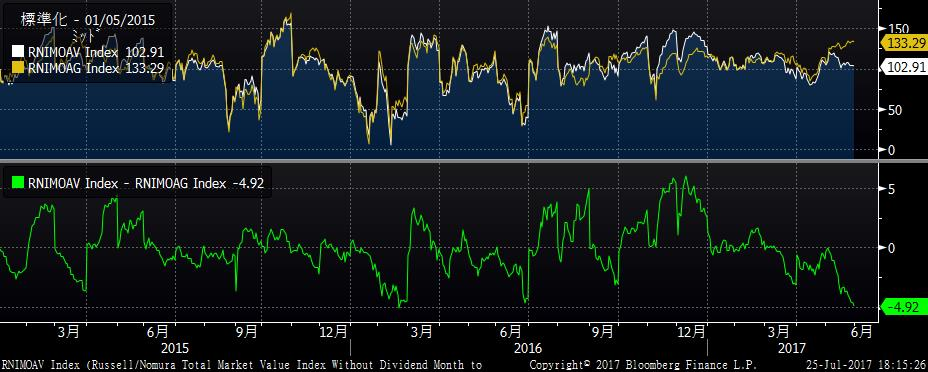
\includegraphics[width=15cm]{./fig/Value.jpg}
		\caption{Russell Nomura日本株インデックス(Value)}
		\label{fig:Value}
	\end{center}
\end{figure}

次に,実際にファクターとして使用する時系列を図\ref{fig:factor_plot}に示した.
また,多重共線性などの問題が無いことを確認するため,散布図とヒストグラム,相関行列を図\ref{fig:factor_cor}にまとめた.図\ref{fig:factor_cor}の対角線上にある図が各ファクターのヒストグラムとカーネル密度関数,下三角の図がファクター間の散布図,上三角の図がファクター間の相関係数に100を掛けた数値を表している.
さらに,ファクターの基本統計量を表\ref{tbl:factor_summary}に示した.
%対数収益率について書いたほうがいいのでは

\begin{figure}[H]
	\begin{center}
		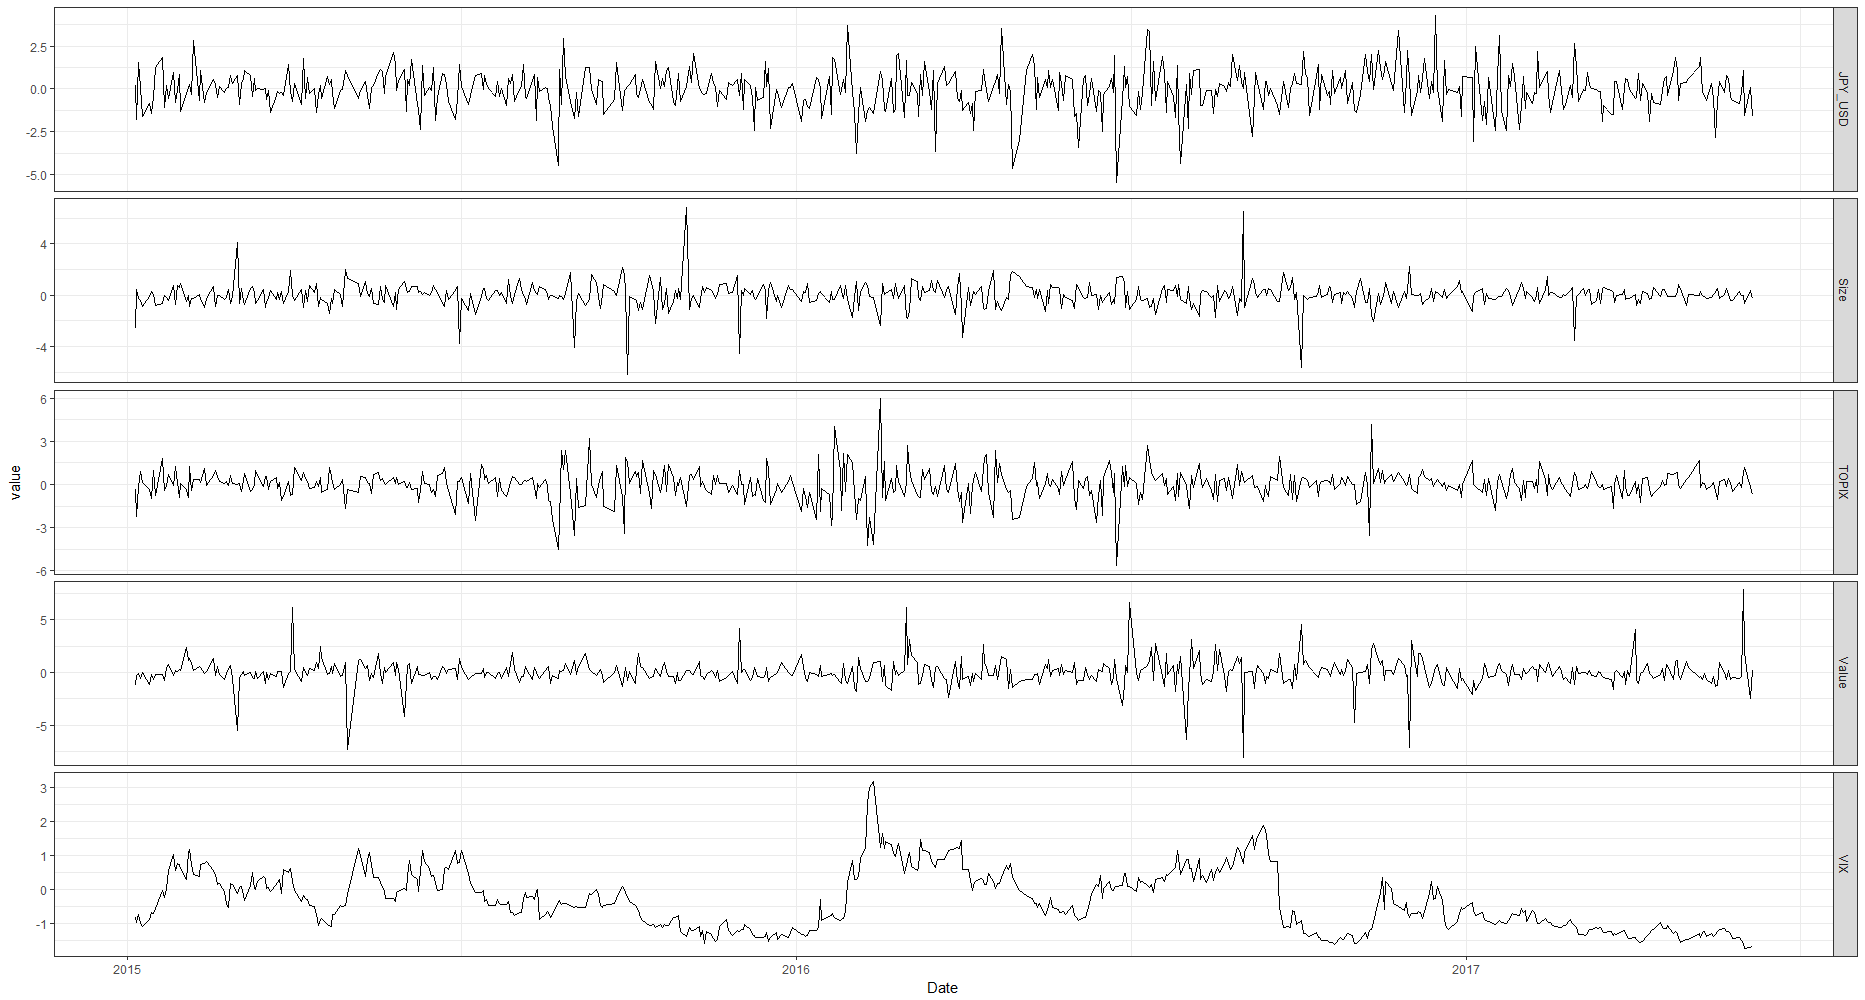
\includegraphics[width=15cm]{./fig/factor_plot.png}
		\caption{ファクターの時系列プロット}
		\label{fig:factor_plot}
	\end{center}
\end{figure}

\begin{figure}[H]
	\begin{center}
		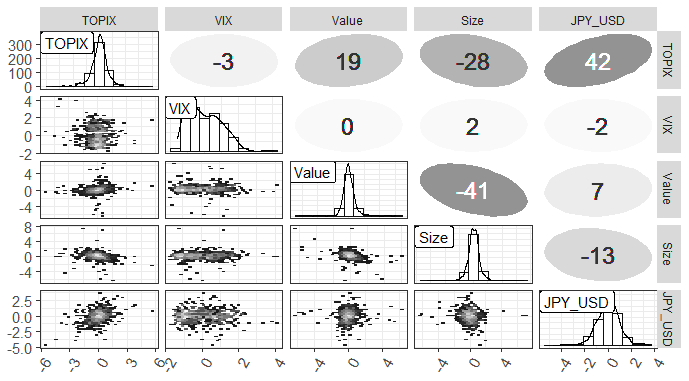
\includegraphics[width=15cm]{./fig/factor_cor.png}
		\caption{ファクター間の相関関係とヒストグラム}
		\label{fig:factor_cor}
	\end{center}
\end{figure}

\begin{table}[H]
\caption{ファクターの基本統計量}
\begin{center}
\begin{tabular}{|c|c|c|c|c|c|}
\hline
統計量 & TOPIX & VIX & Value & Size & JPY$\_$USD\\
\hline
\hline
 Min		&-5.33806&-1.6387&-6.34983&-6.42186&-4.64922\\
 1st Qu	&-0.45082&-0.8659&-0.41889&-0.39178&-0.56066 \\
 Median	&0.05201&-0.1465&-0.06176&0.02299 &0.02342 \\
 Mean		&0.00000&0.0000&0.00000&0.00000&0.00000\\
 3rd Qu 	&0.49170&0.7329&0.38466&0.46966&0.59423\\
 Max		&5.69692&4.1170&6.21356&7.16976&3.67393 \\
\hline
 sd 		&1.00000&1.0000&1.00000&1.00000&1.00000\\

\hline
\end{tabular}
\end{center}
\label{tbl:factor_summary}
\end{table}


図\ref{fig:factor_plot}より,TOPIX, Value, Size, JPY$\_$USDはどれも定常時系列であることが分かる.VIXに関しては,ボラティリティの変化率ではなく,大きさをファクターとして扱うために原系列をそのまま正規化した.そのため明らかに分散が不均一な過程になっている.

次に図\ref{fig:factor_cor}を確認する.TOPIX, Value, Sizeは時折大きな変動を見せるため,中心付近で高く,裾の広い分布になっている.
図\ref{fig:factor_cor}右上の,ファクター間の相関係数を100倍した数値を確認すると,全体的に非常に低い値を取っているが,低い相関を持つファクターの組み合わせが存在することが見て取れる.
この場合TOPIXとJPY$\_$USDの42,ValueとSizeの-41,TOPIXとSizeの-28である.
よって,完全に独立なファクターであるとは言えないまでも,回帰モデルには十分利用可能なファクターであることが確認できた.
モデルのパラメータ推定方法については次節で述べる.


\subsection{ファクターモデルの推定}
モデル推定のための学習期間を3カ月に設定し,推定したモデルでその先1カ月の運用パフォーマンス(バックテスト)を計測する.
この分析を1カ月ごとにローリングしながら推定と計測を繰り返す.
そのイメージ図を以下の図\ref{fig:backtest}に示した.

\begin{figure}[H]
	\begin{center}
		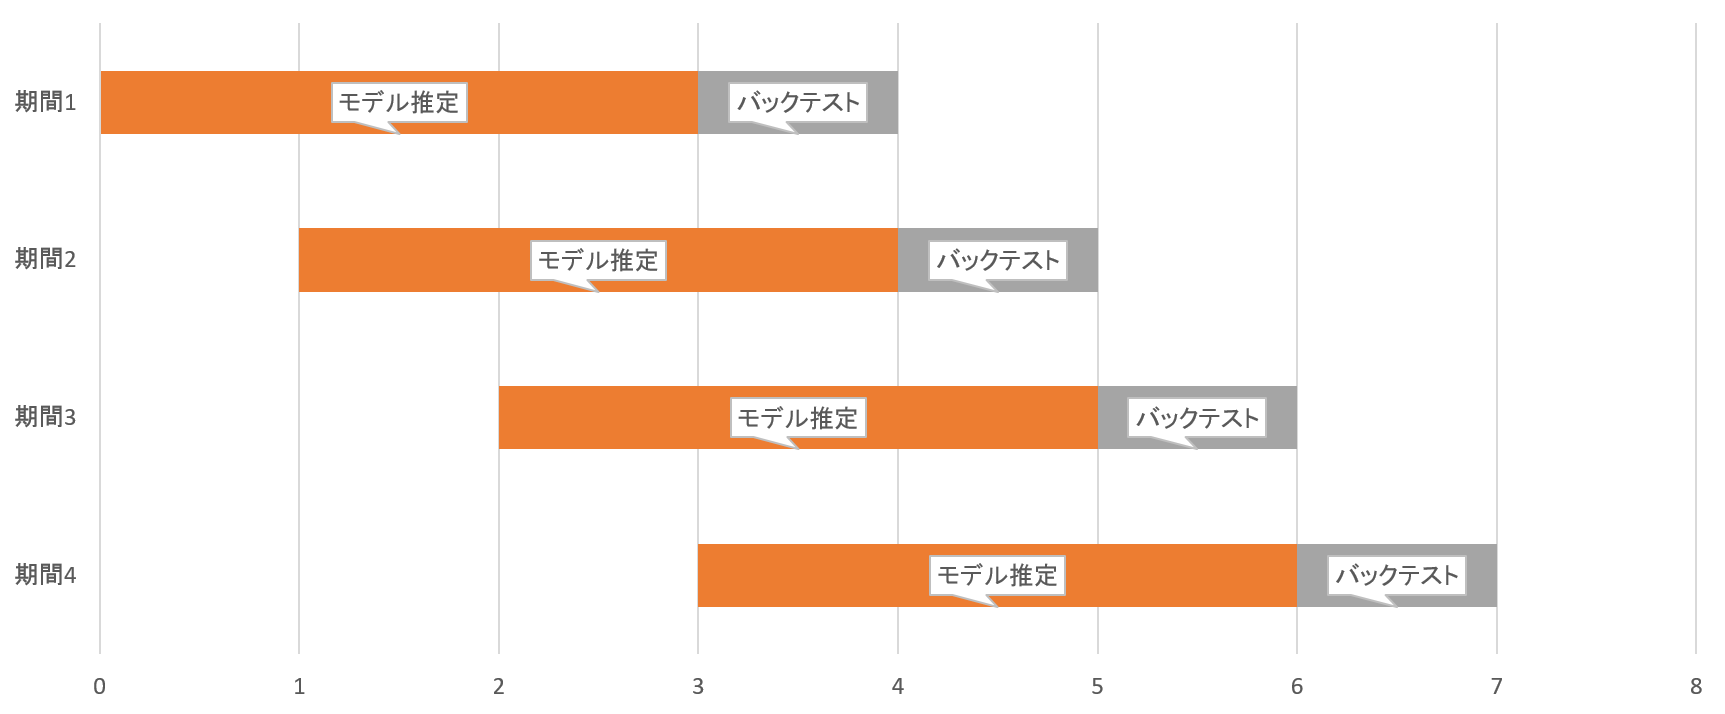
\includegraphics[width=15cm]{./fig/backtest.png}
		\caption{バックテストのイメージ図}
		\label{fig:backtest}
	\end{center}
\end{figure}

%3カ月にする理由が欲しい.

マルチ・ファクターモデルを推定する際,過適合を避けるため,lasso回帰によるモデル推定と変数選択を行った.
lasso回帰は,係数の過大化を防ぎ汎化性能を高めるだけでなく自動的に「変数選択」を行う能力を持て,過適合を避けることが出来る.

$t=1,\cdots,T$の期間において,銘柄$i$のマルチ・ファクターモデルは以下の式を最小化することにより求まる.$\alpha_i$が含まれていないが,これは各推定期間ごとに正規化することによる.
\begin{equation}
\sum_{t=1}^T\left(r_{i,t} - \sum_{k=1}^5\beta_{i,k}F_{k,t} \right)^2 + \lambda_i\sum_{k=1}^5|\beta_{i,k}|
\end{equation}
問題は正則化項のパラメータ$\lambda_i$に関してであるが,これは交差検証法によって最小二乗誤差が最小の値を使用する.今回の分析では交差検証法の分割を全て10とした.

全26期間で行った推定のうち,最初と最後の期間に関する結果を表\ref{tbl:model_summary1}, \ref{tbl:model_summary2}に示した.

\begin{table}[H]
\caption{ファクターモデルの推定結果(訓練期間:2015年1月から3月)}
\begin{center}
\begin{tabular}{|c|c|c|c|c|c|c|}
\hline
 統計量& $\alpha$    &         TOPIX   &             VIX      &        Value   &         Size       &        JPY$\_$USD    \\      
\hline
\hline
 Min&-0.0143864& -0.006802& -0.02629 & -0.01499 &-0.010450 &-0.01182 \\
 1st Qu&-0.0012404 & 0.003709 & 0.00000 &  0.00000 & 0.000000 & 0.00000 \\ 
 Median &-0.0001376 & 0.007552 & 0.00000  & 0.00000 & 0.000000 & 0.00000 \\ 
 Mean   &0.0001227& 0.0074834& 0.0002030& 0.0004132& 0.0011393& 0.0000702  \\
 3rd Qu& 0.0012743 & 0.010987 & 0.00000  & 0.00000 & 0.001281 & 0.00000  \\
 Max  &0.0181611 & 0.028263 & 0.01792  & 0.02979 & 0.037666 & 0.01556 \\
\hline
sd & 0.002412  & 0.005135  & 0.002535 &0.001950 &0.002910 & 0.001690 \\
\hline
\end{tabular}
\end{center}
\label{tbl:model_summary1}
\end{table}


\begin{table}[H]
\caption{ファクターモデルの推定結果(訓練期間:2017年3月から5月)}
\begin{center}
\begin{tabular}{|c|c|c|c|c|c|c|}
\hline
 統計量& $\alpha$   &         TOPIX   &             VIX      &        Value   &         Size       &        JPY$\_$USD    \\      
\hline
\hline
 Min&-0.0311943 &0.000000&-0.027704 & -0.02503& -0.010465& -0.008442 \\
 1st Qu&-0.0003752 & 0.005102 & 0.000000  & 0.00000 & 0.000000 & 0.000000 \\ 
 Median &0.0009955 &0.008934 & 0.000000  & 0.00000 & 0.000000 & 0.000000 \\ 
 Mean   &2.361e-03 & 8.874e-03 & 1.459e-03 & 6.364e-06 & 1.335e-03 & 1.654e-04   \\
 3rd Qu&0.0036495 & 0.012430 & 0.001103  & 0.00000 & 0.002435 & 0.000000  \\
 Max   &0.0587778 & 0.028889 & 0.044701  & 0.01014 & 0.016323 & 0.012010 \\
\hline
sd &  0.006413 & 0.005366 & 0.005131 & 0.001808 & 0.002374&  0.001316 \\
\hline
\end{tabular}
\end{center}
\label{tbl:model_summary2}
\end{table}

表\ref{tbl:model_summary1},\ref{tbl:model_summary2}より,TOPIX以外のファクターに対する感度では,第1四分位点や中央値,第3四分位点で0となっているものがある.
これはlasso回帰による結果であり,変数選択とパラメータ推定が同時に行えていることによる.
一方TOPIXに対する感度ではそのようなことはなく,市場ポートフォリオのファクターとしての重要さが伺える.

%最適化の話かく???
\subsection{リスク・プレミアム}
過去3ヶ月のデータより推定したマルチ・ファクターモデルに基づいて算出したリスク・プレミアムを以下の図\ref{fig:riskpremium}に示した.具体的には,2.6節の式(\ref{eq:fp})を一般化逆行列を利用することによりファクター・ポートフォリオを推定し,その期待収益率をファクターのリスク・プレミアムとした.

\begin{figure}[H]
	\begin{center}
		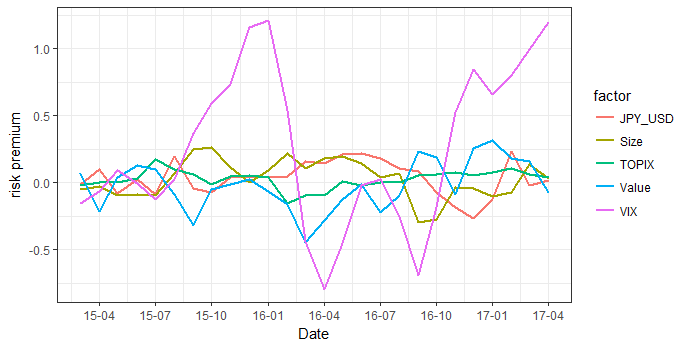
\includegraphics[width=15cm]{./fig/riskpremium.png}
		\caption{リスク・プレミアムの推移}
		\label{fig:riskpremium}
	\end{center}
\end{figure}

図\ref{fig:risk_premium}より,リスク・プレミアムの中には0以下になるものがある.全てのファクターに,常にリスクを取る「価値」があるわけではないことが分かる.

\subsection{様々なポートフォリオ}

本レポートで取り入れたファクターが,CAPMにおけるアノマリーを説明できているかを確かめるため,推定したマルチ・ファクターモデルの各係数(ベータ)の上位30銘柄で等加重ポートフォリオを作成した.また,その累計リターンの推移を以下の図\ref{fig:factor_top30}に示した.また,市場ポートフォリオに対してのパフォーマンスを確認するために,TOPIXの累計リターンをbenchmarkとして共に示した.


\begin{figure}[H]
	\begin{center}
		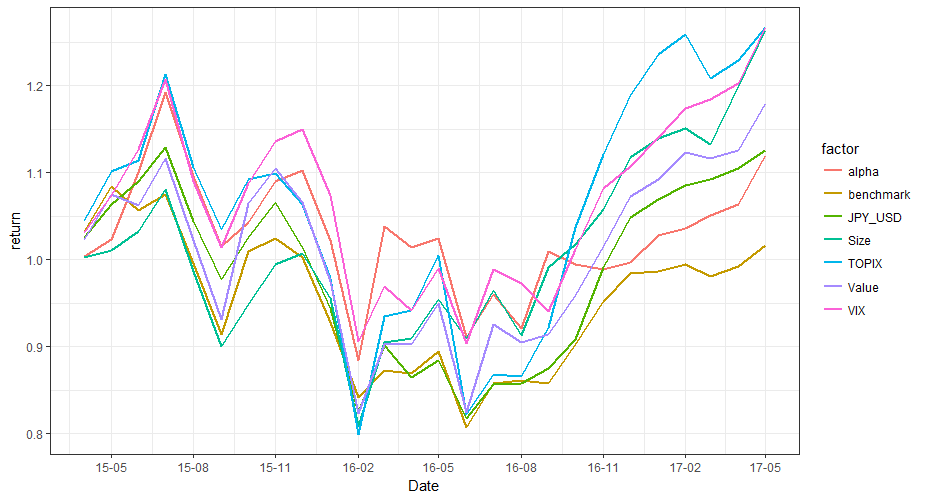
\includegraphics[width=15cm]{./fig/factor_top30.png}
		\caption{各ベータ上位30銘柄による等加重ポートフォリオ}
		\label{fig:factor_top30}
	\end{center}
\end{figure}


図\ref{fig:factor_top30}より,どのポートフォリオも似たような動きをしており,市場ポートフォリオの影響力が非常に大きいことが分かる.
各ポートフォリオのトータル・リターンは以下のようである.

\begin{table}[H]
\begin{center}
\begin{tabular}{|c|c|c|c|c|c||c|}
\hline
 Alpha  &    TOPIX   &             VIX      &        Value   &         Size       &        JPY$\_$USD &Benchmark   \\      
\hline
1.1200443 & 1.26693 & 1.26658  &  1.17973 & 1.26378 & 1.12613 & 1.01636\\
\hline
\end{tabular}
\end{center}
\caption{各ベータ上位30銘柄による等荷重ポートフォリオ}
\label{tbl:factor_top30}
\end{table}


表\ref{tbl:factor_top30}より,最もリターンの低いポートフォリオは市場ポートフォリオであり,2番目に低いポートフォリオは期待収益率上位30銘柄による等荷重ポートフォリオである.これにより,市場ポートフォリオだけでは説明のつかないアノマリーの存在をマルチ・ファクターモデルによって抜き出せていることが確認できた.

\subsection{ポートフォリオ選択}

ポートフォリオの収益率ファクターに対する感度は2.2節の式(\ref{eq:multi})により与えられていた.今回は5ファクターモデルを考えているため,ポートフォリオの収益は次のように与えられる.
\begin{equation}
\begin{split}
R_P &= \alpha_P + \beta_{P,1} F_1 + \beta_{P,2} F_2 + \cdots + \beta_{P,5} F_m + \varepsilon_P\\
&=\sum_{i=1}^N \alpha_i + F_1 \sum_{i=1}^N w_i \beta_{i,1} + \cdots + F_5 \sum_{i=1}^N w_i \beta_{i,m} + \sum_{i=1}^N w_i\varepsilon_i\\
&= \sum_{i=1}^N \alpha_i + \sum_{k=1}^5 \sum_{i=1}^N w_i \beta_{i,k} F_k + \sum_{i=1}^N w_i\varepsilon_i
\label{eq:port}
\end{split}
\end{equation}

リスク・プレミアムを算出したことによりファクターごとのリスクを取る価値が定量化できたのであった.
ここで,負のリスク・プレミアムを持つに対しては分散化し,より高いリスク・プレミアムを持つファクターに対してはエクスポージャーするようなポートフォリオ構築を目指す.
10$\sim$30銘柄に絞り込まなければならないので以下の手法により銘柄を選定した.
また,リスク・プレミアムが負であるファクターに対し分散化する目的で,等荷重ポートフォリオを構成した.

\begin{itembox}[l]{ポートフォリオ選択の手順}
\begin{enumerate}
\item 直近3ヶ月のデータより推定したファクターごとのリスク・プレミアムのうち,最もプレミアムの大きいファクターへの感度が高いもの上位100銘柄を選択する.
\item 1で選択した100銘柄のうち,期待収益率が高い30銘柄を選択
\item 2で選択した30銘柄により等加重ポートフォリオを構成
\end{enumerate}
\end{itembox}

この手法を用いて行ったバックテストの結果を以下の図\ref{fig:teiann}に示した.

\begin{figure}[H]
	\begin{center}
		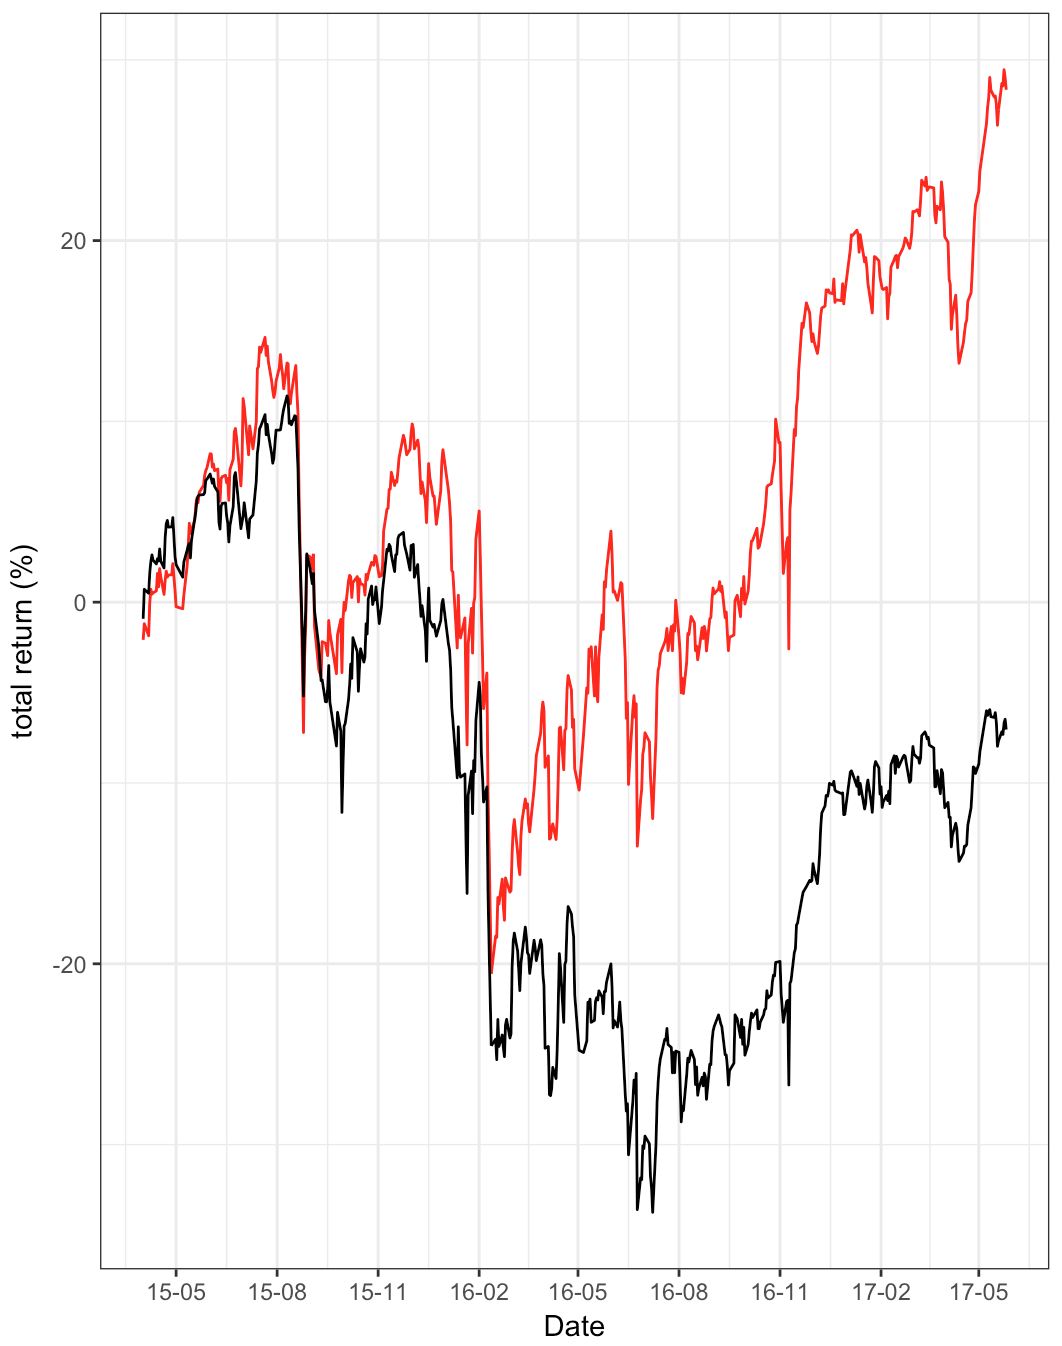
\includegraphics[width=15cm]{./fig/teiann.png}
		\caption{提案手法によるバックテスト}
		\label{fig:teiann}
	\end{center}
\end{figure}

提案した手法のトータルリターンは,バックテストを行った26カ月間で約34.4\%であった.
これはベンチマークであるTOPIX(東証株価指数)を約32.8\%アウトパフォームしている.
図\ref{fig:factor_top30}で示したように単にアルファやベータの高い銘柄を選ぶのではなく,ファクターのリスク・プレミアムによる選択を行った結果である.
図\ref{fig:factor_top30}の結果と見比べると,ベータを追うだけでなくファクターのリスク・プレミアム,つまりファクターにエクスポージャーする「価値」を追う事の意義が伺える.

\section{途中経過}
コンテストの測定期間は2017年7月から8月末にかけてであるが,本レポートの提出期限が2017年7月末であるため,7月末時点での結果を述べる.
提出したポートフォリオの構成とそのリターンを示し,リバランスの内容にも触れる.
\subsection{提出したポートフォリオ}
3.6節で提案した手順に基づいて,提出するポートフォリオを決定した.
本コンテストのパフォーマンス計測は2017年7月3日より始まるため,2017年4月3日から2017年6月29日にかけてデータを取得し,3章と同様の分析を行った.
提案した手法により選択された銘柄とそのウェート,時価総額を表\ref{tbl:port1}に示した.
また,ポートフォリオ登録時点では等荷重ポートフォリオを構築したが,7月3日までの価格変動により若干のズレが生じている.

\begin{table}[htbp]
\caption{提出したポートフォリオ}
\begin{center}
\begin{tabular}{|c|c|c|}
\hline
企業名 & ウェート(\%) & 時価総額(円, 7月3日時点)\\
\hline
\hline
グローブライド	&3.34&3,343,642\\
コメダホールディングス&3.33	&3,335,200\\
ゼンショーホールディングス&3.33&	3,339,875\\
三井ホーム&3.33&3,333,333\\
井筒屋&3.33	&3,341,014\\
日成ビルド工業&3.35&3,360,302\\
美津濃&3.28	&3,287,108\\
藤倉ゴム工業	&	3.36	&	3,369,011	\\
近鉄百貨店	&	3.35	&	3,352,435	\\
GSIクレオス	&	3.30	&	3,309,523	\\
イマジカ・ロボット・ホールディングス	&	3.34	&3,351,877\\
グランディハウス	&	3.30	&	3,309,859	\\
サンフロンティア不動産	&	3.43	&	3,432,881	\\
北陸電力	&	3.32	&	3,326,772	\\
アイ・オー・データ機器	&	3.35	&	3,360,768	\\
アドソル日進	&	3.36	&	3,363,838	\\
システムリサーチ	&	3.36	&	3,363,148	\\
ルネサスイーストン	&	3.36	&	3,367,816	\\
日本電波工業	&	3.36	&	3,363,984	\\
ソフトクリエイトホールディングス	&	3.35	&3,361,324\\
カワチ薬品	&	3.35	&	3,353,240	\\
三井製糖	&	3.39	&	3,395,734	\\
六甲バター	&	3.30	&	3,305,533	\\
森永乳業	&	3.23	&	3,234,511	\\
養命酒製造	&	3.31	&	3,317,285	\\
ニチハ	&	3.34	&	3,350,168	\\
三井住友建設	&	3.30	&	3,306,233	\\
太平洋興発	&	3.33	&	3,333,333	\\
極東証券	&	3.28	&	3,285,697	\\
SOMPOホールディングス	&	3.35	&	3,353,441\\
\hline
\hline
合計& 100.00 &  100,208,884\\
\hline
\end{tabular}
\end{center}
\label{tbl:port1}
\end{table}


\subsection{7月中のパフォーマンス}

提出したポートフォリオの,トータルリターンの推移を図\ref{fig:totalreturn}に示した.また,東証一部上場銘柄を対象ユニバースとしたため,TOPIXをベンチマークとして合わせて示した.図\ref{fig:totalreturn}の上段がそれぞれのトータルリターンであり,下段がそのパフォーマンス差である.

\begin{figure}[htbp]
	\begin{center}
		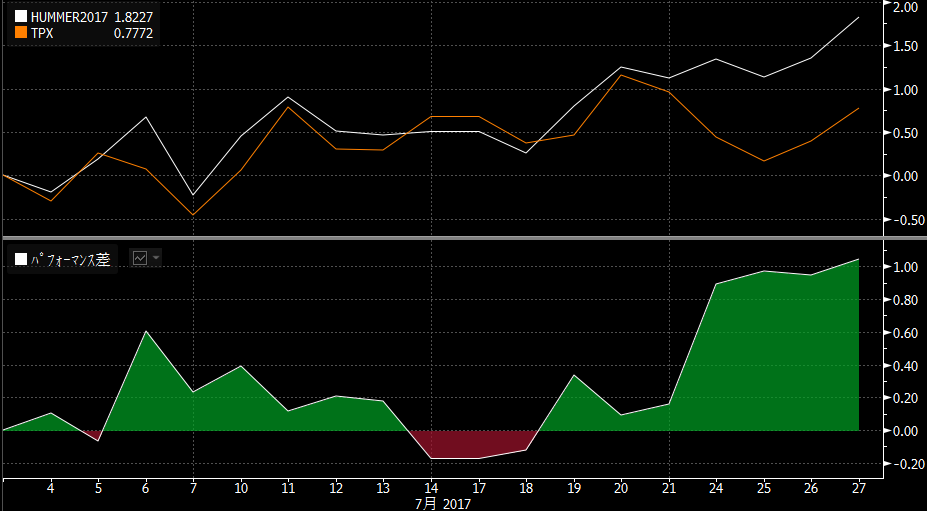
\includegraphics[width=15cm]{./fig/totalreturn.png}
		\caption{7月中のリターン}
		\label{fig:totalreturn}
	\end{center}
\end{figure}

2017年7月3日の終値を基準とすると,TOPIXのトータルリターンが0.7772\%であるのに対し,提出したポートフォリオのトータルリターンは1.8227\%であった.
ベンチマークを1.0455\%アウトパフォームしており,少なくとも2017年7月では提案した手法が有効であったことが確認できる.


\subsection{リバランス}
本コンテストのルールにより,リバランスは7月中に一度しか行えない.
そのため,提案した手法の効果を安定的に得るため,リバランスは7月31日に行うものとした.
1度目のポートフォリオ提出と同様の手法で銘柄を選択し,等荷重ポートフォリオを再構築した.
選択した銘柄とウェート,時価総額を次ページの表\ref{tbl:port2}に示した.
\begin{table}[htbp]
\caption{リバランスしたポートフォリオ}
\begin{center}
\begin{tabular}{|c|c|c|}
\hline
ティッカー & ウェート(\%) & 時価総額(7月31日時点)\\
\hline
\hline
シュッピン & 3.33 & 3366478.87\\
ゼンリン & 3.33 & 3366478.87\\
ラウンドワン & 3.33 & 3366478.87\\
IBJ & 3.33 & 3366478.87\\
RS Technologies & 3.33 & 3366478.87\\
アイ・エス・ビー & 3.33 & 3366478.87\\
ネクシィーズグループ & 3.33 & 3366478.87\\
リブセンス & 3.33 & 3366478.87\\
三井ハイテック & 3.33 & 3366478.87\\
八洲電機 & 3.33 & 3366478.87\\
山一電機 & 3.33 & 3366478.87\\
日本シイエムケイ & 3.33 & 3366478.87\\
第一精工 & 3.33 & 3366478.87\\
プリマハム & 3.33 & 3366478.87\\
北の達人コーポレーション & 3.33 & 3366478.87\\
大光 & 3.33 & 3366478.87\\
神戸物産 & 3.33 & 3366478.87\\
ヨシムラ・フード・ホールディングス & 3.33 & 3366478.87\\
アウトソーシング & 3.33 & 3366478.87\\
イトーキ & 3.33 & 3366478.87\\
クイック & 3.33 & 3366478.87\\
ニッカトー & 3.33 & 3366478.87\\
ライク & 3.33 & 3366478.87\\
丸和運輸機関 & 3.33 & 3366478.87\\
島精機製作所 & 3.33 & 3366478.87\\
日本道路 & 3.33 & 3366478.87\\
プレステージ・インターナショナル& 3.33 & 3366478.87\\
ビジョン & 3.33 & 3366478.87\\
リニカル & 3.33 & 3366478.87\\
EPSホールディングス & 3.33 & 3366478.87\\

\hline
\hline
合計& 100.00 &  100994370\\
\hline
\end{tabular}
\end{center}
\label{tbl:port2}
\end{table}

\section{今後の課題と感想}
\subsection{今後の課題}
間に合わなかった分析や,提出後に浮かんできた疑問点,考えうる批判など数々の課題がある.ここではそれらを列挙する.

\begin{itemize}
\item{データに関する問題}\\
\quad 3.1節で述べたように,2015年からの日次データを取得した.この取得を日次ではなく,前場の終値,後場の終値ごとに取得すれば絶対的に標本数が増え,より精度の高い分析が行えるだろう.
\item{ファクター選択に関する問題}\\
\quad 今回のリサーチでは,3.1節で述べたように使用するファクターを選択した.
その存在が確実といわれるファクターだけでなく,独自のファクターを定性的な理由により取り入れた.
しかし3.2節で述べたように,正規化したファクター間には弱い相関が存在するものがあった.
本来ファクター同士は完全に直交していることが望ましく,統計的な因果推論などを行い適切なファクターの組み合わせ選択を行う必要性があるだろう.

\item{マルチ・ファクターモデル推定に関する問題}\\
\quad 3.3節で述べたように,マルチ・ファクターモデルの推定では工夫をした.
銘柄の中には,lassoによってマーケット・ファクターやサイズ・ファクターなど,その存在が確実とされているファクターへの感度が$0$と推定されたものがあった.
説明力や汎化性能を高めるためとはいえ,このように絶対的なファクターを蔑ろにしてしまうことには議論の余地があるだろう.

\quad また,モデル推定に用いたデータは直近3ヶ月間のものであり,1ヶ月単位で(1月$\sim$3月,2月$\sim$4月,というような)推定を行った.例えばこの期間を2ヶ月間,4ヶ月間,5ヶ月間と変更し同様の作業を行うことで,どのような変化があるのか検証する必要がある.さらに推定を1ヶ月単位で行うのではなく,1日単位で行った場合に関しても検証する必要があるだろう.
\item{リスク・プレミアム推定に関する問題}\\
\quad 上記のように1日単位でモデル推定を行うことにより,それに基づく各ファクターのリスク・プレミアムの推移はより滑らかになることが考えられる.
たとえそうでなかったとしても,データの数が増えることにより新たな発見につながると予想できる.

\quad また,ボラティリティ・ファクターのプレミアムの分散は他に比べて非常に大きいものとなっていた.このことは直感に反しており,さらに考察をしていく必要があると感じた.さらに,ファクターのリスク・プレミアム同士がお互いに影響を及ぼしているかについても分析することが出来るだろう.

\item{ポートフォリオ選択に関して}\\
\quad リスク・プレミアムが負であるファクターに関して,感度が0であるポートフォリオを構築することが目的の一つであった.多目的最適化を考えることにより,価値のあるファクターにエクスポージャーするだけでなく,高度に最適化されたポートフォリオを考えることが出来るだろう.ただし,計算時間の観点より,適切なアプローチをとらなければならないだろう.


\end{itemize}

\newpage

\begin{thebibliography}{30}
	\bibitem{analyst} 小林孝雄,芹田敏夫,日本証券アナリスト協会『新・証券投資理論I 理論篇』(日本経済新聞出版社,2009)
	\bibitem{finance} デービッド・G・ルーエンバーガー『金融工学入門』(日本経済新聞社,2002)
	\bibitem{Basu} Basu, S. ''Investment Performance of Commin Stocks in Relation to their Price-Earnings Ratios'', Journal of Finance, 663-682(1977)
	\bibitem{Banz} Banz, R.W. ''The relationship between return and market value of common stock'', Journal of Financial Economics, 3-18(1981)
	\bibitem{Fama} Fama, E.F. and K.R. French ''Common risk factors in the returns on stocks and bonds'', Journal of Financial Economics, 33, 3-56(1993)
	\bibitem{Jagadeesh} Jagadeesh, N. and Titman, S. ''Returns to Buying Winners and Selling Losers: Implications for Stock Market Efficiency.'', Journal of Finance 48, 65–91(1993)
	\bibitem{Ross} Ross, S. ''The Arbitrage Theory of Capital Asset Pricing'', Journal of Economic Theory 13, 341-360(1976)
	
\end{thebibliography}
\end{document}



%表を載せる
%表目次,図目次書き方
%引用の仕方
%目次は提出するのか

%テーマ
